\chapter{Tutorial}
\label{chapter-Tutorial}

This appendix serves as an introduction to the \emph{Workflow Definition API}
and \emph{Workflow Execution API} (see Figure \ref{figure-architecture}).

\section{Workflow Definition API}

\subsection{Defining a New Workflow}

In this subsection, we define a new workflow by creating an object graph of
\texttt{ezcWorkflowNode} objects. Once we learned how to define and store such
a workflow definition, we we will look at loading and editing an existing
workflow definition.

\subsubsection{Creating the Object Graph}

First, we load the \texttt{ezcBase} component (line 2) and set up its
classloader that is based on PHP's \texttt{\_\_autoload} interceptor
(lines 4--7).

\begin{lstlisting}[language=PHP,firstnumber=1]
<?php
require_once 'Base/base.php';

function __autoload( $className )
{
    ezcBase::autoload( $className );
}
\end{lstlisting}

For the following code listings, lines 1--7 will always be the same as in the
listing above.

We create a new object of the \texttt{ezcWorkflow} class (line 8). This object
represents the workflow that we are about to define. The constructor of the
class expects a string with a name for the workflow. This name is unique for
the schema repository to which the workflow may be saved later.

\begin{lstlisting}[language=PHP,firstnumber=8]
$workflow = new ezcWorkflow( 'Test' );
\end{lstlisting}

We define an \emph{Input} node by creating an object of the
\texttt{ezcWorkflowNodeInput} class. The constructor expects an associative
array where the key stands for the name of an input variable and the value
may hold arbitrary expectations for this variable. These expectations are
evaluated and checked by the application that uses the workflow component.

Then we set up the \emph{Input} node as an outgoing node of the \emph{Start}
node.

\begin{lstlisting}[language=PHP,firstnumber=9]
$input = new ezcWorkflowNodeInput(
  array(
    'choice' => new ezcWorkflowConditionIsBool
  )
);

$workflow->startNode->addOutNode( $input );
\end{lstlisting}

For the purposes of this example we assume that \texttt{'choice' => 'boolean'}
means that a boolean input variable of name ''choice'' is expected.

We now define an \emph{Exclusive Choice} node that uses the value of the input
variable to activate one of two possible paths. Before we set up its outgoing
nodes (and the related conditions), we set up the \emph{Exclusive Choice} as
an outgoing node of the \emph{Input} node (lines 16--17).

\begin{lstlisting}[language=PHP,firstnumber=16]
$branch = new ezcWorkflowNodeExclusiveChoice;
$branch->addInNode( $input );
\end{lstlisting}

In the next step, we create two objects, \texttt{\$true} and \texttt{\$false}
of the \texttt{ezcWorkflowNodeAction} class (lines 18--19). The constructor
expects the name of a class that implements the\\ \texttt{ezcWorkflowServiceObject}
interface. Such a class encapsulates the business logic that is associated with the
\emph{Action} node.

\begin{lstlisting}[language=PHP,firstnumber=18]
$true  = new ezcWorkflowNodeAction( 'PrintTrue' );
$false = new ezcWorkflowNodeAction( 'PrintFalse' );
\end{lstlisting}

Let us take a look at what an implementation of the
\texttt{ezcWorkflowServiceObject} interface looks like:

\begin{quote}
\begin{lstlisting}[language=PHP,firstnumber=1,stepnumber=100]
<?php
class PrintTrue implements ezcWorkflowServiceObject
{
    public function execute( ezcWorkflowExecution $e )
    {
        print "TRUE\n";
    }

    public function __toString()
    {
        return 'PrintTrue';
    }
}
?>
\end{lstlisting}

The \texttt{ezcWorkflowServiceObject} interface requires two methods,
\texttt{execute()} and \texttt{\_\_toString()}. The former implements the
business logic of the service object and is passed the execution context as
its only argument. The latter provides a textual representation of the
service object.
\end{quote}

Using the \texttt{\$branch} object's \texttt{addConditionalOutNode()} method,
we can now set up the \emph{Action} node that is represented by the
\texttt{\$true} object as an conditional outgoing node (lines 20--26). This
method expects an \texttt{ezcWorkflowCondition} object as its first argument.
This object encapsulates the branching condition.

For our example we use the \texttt{ezcWorkflowConditionIsTrue} class. The
constructor of this class expects the name of a workflow variable that is to
be evaluated.

\begin{lstlisting}[language=PHP,firstnumber=20]
$branch->addConditionalOutNode(
  new ezcWorkflowConditionVariable(
    'choice',
    new ezcWorkflowConditionIsTrue
  ),
  $true
);
\end{lstlisting}

Section~\ref{section-ConditionClasses} shows the available
\texttt{ezcWorkflowCondition} implementations.

Analogous, we set up the \emph{Action} node that is represented by the
\texttt{\$false} object as a second conditional outgoing node (lines 27--33).

\begin{lstlisting}[language=PHP,firstnumber=27]
$branch->addConditionalOutNode(
  new ezcWorkflowConditionVariable(
    'choice',
    new ezcWorkflowConditionIsFalse
  ),
  $false
);
\end{lstlisting}

Finally, we create a new object of the \texttt{ezcWorkflowNodeSimpleMerge}
class (line 34). We set up the two \emph{Action} nodes as incoming nodes and the
\emph{End} node as an outgoing node of this \emph{Simple Merge} node (lines 35--37).

\begin{lstlisting}[language=PHP,firstnumber=34]
$merge = new ezcWorkflowNodeSimpleMerge;
$merge->addInNode( $true )
      ->addInNode( $false )
      ->addOutNode( $workflow->endNode );
\end{lstlisting}

This concludes the creation of the object graph that represents the workflow
specification and can now be stored in a workflow schema repository. Currently
two workflow schema repository backends are supported, XML files and relational
databases.

\subsubsection{Writing the Workflow Schema to an XML File}

The following code snippet demonstrates how to serialize the object graph to
an XML representation.

\begin{lstlisting}[language=PHP,firstnumber=38]
$definition = new ezcWorkflowDefinitionStorageXml;
$definition->save( $workflow );
?>
\end{lstlisting}

The constructor of the \texttt{ezcWorkflowDefinitionStorageXml} class accepts an
optional argument that specifies the directory in which the XML files are
stored.

Listing \ref{listing-XML2} shows the resulting XML document that is written to
a file named \texttt{Test\_1.xml}. The filename includes the name of the
workflow definition and its version number.

\begin{lstlisting}[language=XML,firstnumber=1,stepnumber=100,float,caption={Workflow specification in XML markup},label=listing-XML2]
<?xml version="1.0" encoding="UTF-8"?>

<workflow name="Test" version="1">
  <node id="1" type="Start">
    <outNode id="3"/>
  </node>

  <node id="2" type="End"/>

  <node id="3" type="Input">
    <variable name="choice">
      <condition type="IsBool"/>
    </variable>
    <outNode id="4"/>
  </node>

  <node id="4" type="ExclusiveChoice">
    <condition type="Variable" name="choice">
      <condition type="IsTrue"/>
      <outNode id="5"/>
    </condition>

    <condition type="Variable" name="choice">
      <condition type="IsFalse"/>
      <outNode id="6"/>
    </condition>
  </node>

  <node id="5" type="Action" serviceObjectClass="PrintTrue">
    <outNode id="7"/>
  </node>

  <node id="6" type="Action" serviceObjectClass="PrintFalse">
    <outNode id="7"/>
  </node>

  <node id="7" type="SimpleMerge">
    <outNode id="2"/>
  </node>
</workflow>
\end{lstlisting}

Frontend languages such as the XML Process Definition Language (XPDL)
\cite{WfMC05} can be transformed to this format using XSL Transformations
(XSLT) \cite{W3C07}, for instance.

\subsubsection{Saving the Workflow Schema to a Database}

The constructor of the \texttt{ezcWorkflowDatabaseDefinition} class expects
and object of the \texttt{ezcDbHandler} class. In line 38 we create such an
object and connect to a MySQL database server. Then we can use the
\texttt{save()} method of the \texttt{ezcWorkflowDatabaseDefinition} object
to save the object graph to the database.

\begin{lstlisting}[language=PHP,firstnumber=38]
$db         = ezcDbFactory::create( 'mysql://test@localhost/test' );
$definition = new ezcWorkflowDatabaseDefinition( $db );
$definition->save( $workflow );
?>
\end{lstlisting}

\subsubsection{Visualizing a Workflow Graph}

The next code snippet shows how to use the \texttt{ezcWorkflowVisitorVisualization}
class to generate a description of the object graph in the DOT graph description
language.

\begin{lstlisting}[language=PHP,firstnumber=38]
$visitor = new ezcWorkflowVisitorVisualization;
$workflow->accept( $visitor );
print $visitor;
?>
\end{lstlisting}

Listing~\ref{listing-DOT} shows the resulting DOT graph description,
Figure~\ref{figure-GraphVizExample} shows the workflow graph rendered using
GraphViz from this graph description.

\begin{lstlisting}[firstnumber=1,stepnumber=100,float,caption={Workflow specification in DOT markup},label=listing-DOT]
digraph Test {
node1 [label="Start"]
node3 [label="Input"]
node4 [label="Exclusive Choice"]
node5 [label="PrintTrue"]
node7 [label="Simple Merge"]
node2 [label="End"]
node6 [label="PrintFalse"]

node1 -> node3
node3 -> node4
node4 -> node5 [label="choice is true"]
node4 -> node6 [label="choice is false"]
node5 -> node7
node7 -> node2
node6 -> node7
}
\end{lstlisting}

\begin{figure}[hbt]
\begin{center}
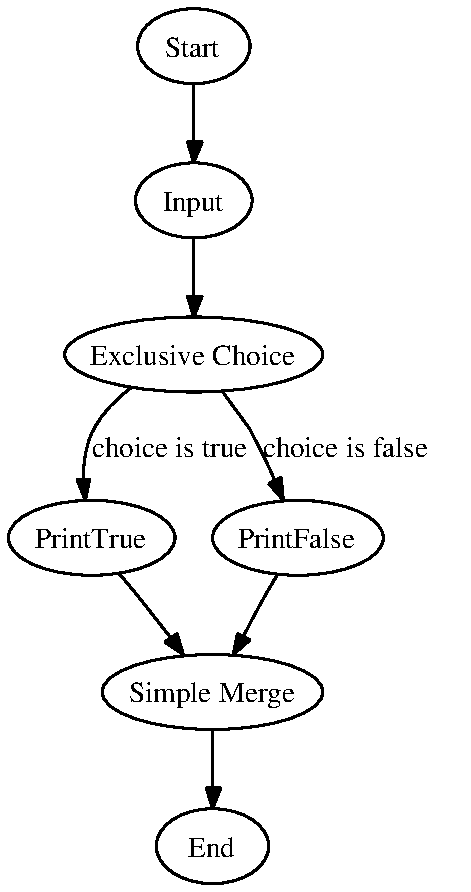
\includegraphics[width=7cm]{figures/GraphVizExample}\\[5mm]
\end{center}
\caption{Workflow graph rendered using GraphViz}
\label{figure-GraphVizExample}
\end{figure}

\subsection{Loading an Existing Workflow}

\subsubsection{Loading a Workflow Schema from an XML File}

The following code snippet demonstrates how to load an object graph from
an XML representation.

\begin{lstlisting}[language=PHP,firstnumber=8]
$definition = new ezcWorkflowDefinitionStorageXml;
$workflow   = $definition->loadByName( 'Test' );
?>
\end{lstlisting}

The \texttt{loadByName()} method accepts an optional second argument that
specifies the version number of the workflow definition that is to be loaded.
By default (ie. without the second argument) the newest version of the workflow
is loaded.

\subsubsection{Loading a Workflow Schema from a Database}

Loading a workflow schema from a database is analogous to loading fron an XML
file:

\begin{lstlisting}[language=PHP,firstnumber=8]
$db         = ezcDbFactory::create( 'mysql://test@localhost/test' );
$definition = new ezcWorkflowDatabaseDefinition( $db );
$workflow   = $definition->loadByName( 'Test' );
\end{lstlisting}

For the following code listings, lines 8--10 will always be the same as in the
listing above.

\section{Workflow Execution API}

The software that has been developed as part of this thesis offers three
workflow execution engines: \texttt{ezcWorkflowExecutionNonInteractive},
\texttt{ezcWorkflowDatabaseExecution}, and \texttt{ezcWorkflowTestExecution}.
This sections shows how they are used.

\subsection{Workflow with Wait States}

For the execution of a workflow that contains wait states (for example
\emph{Input} nodes), an execution engine is required that supports
persistence. The \texttt{ezcWorkflowDatabaseExecution} class implements
such an execution engine and uses a relational database for persistence
storage.

In the following code snippet we start start the execution of a previously
loaded workflow.

\begin{lstlisting}[language=PHP,firstnumber=11]
$execution = new ezcWorkflowDatabaseExecution( $db );
$execution->workflow = $workflow;
$executionId = $execution->start();
\end{lstlisting}

As our workflow contains an \emph{Input} node, the execution will not complete
and will be suspended. The \texttt{\$executionId} uniquely identifies the
suspended workflow execution. It can be used, for instance, to resume the
workflow execution once the requested input data has been provided:

\begin{lstlisting}[language=PHP,firstnumber=14]
$execution = new ezcWorkflowDatabaseExecution( $db );
$execution->resume( $executionId, array( 'choice' => true ) );
?>
\end{lstlisting}

\subsection{Workflow without Wait States}

A workflow that contains no wait states can be executed in one pass. The
workflow engine is not required to support persistence for this. The
\texttt{ezcWorkflowExecutionNonInteractive} class implements a workflow
engine without persistence support that can execute such workflow without
the overhead of a persistence layer.

\begin{lstlisting}[language=PHP,firstnumber=11]
$execution = new ezcWorkflowExecutionNonInteractive;
$execution->workflow = $workflow;
$execution->start();
?>
\end{lstlisting}

\subsection{Simulating Workflow Execution}

The workflow engine implemented by the \texttt{ezcWorkflowTestExecution}
class can be used for testing both the workflow system itself as well as
workflow definitions.

\begin{lstlisting}[language=PHP,firstnumber=11]
$execution = new ezcWorkflowTestExecution;
$execution->workflow = $workflow;
$execution->setInputVariable( 'choice', true );
$execution->start();
?>
\end{lstlisting}

The \texttt{setInputVariable()} method allows for the mocking of
\emph{Input} nodes, thus making it possible to execute and test interactive
workflows without interaction.
